\documentclass[conference]{IEEEtran}
\IEEEoverridecommandlockouts
\usepackage[T1]{fontenc}
\usepackage{cite}
\usepackage{amsmath,amssymb,amsfonts}
\usepackage{graphicx}
\usepackage{algorithm}
\usepackage{algorithmic}
\usepackage{textcomp}
\usepackage{xcolor}
\usepackage{balance}
\usepackage{multirow}
\usepackage{booktabs}
\usepackage{caption}
\usepackage{subfig}
\usepackage{hyperref}
\hypersetup{hidelinks}
\usepackage{tikz}
\usetikzlibrary{positioning, arrows.meta, shapes.geometric, fit, calc, shadows}

\def\BibTeX{{\rm B\kern-.05em{\sc i\kern-.025em b}\kern-.08em
    T\kern-.1667em\lower.7ex\hbox{E}\kern-.125emX}}

\pagestyle{plain}

\begin{document}

\title{A Two-Stage Raspberry Pi Security Pipeline\\for Military IoT Attack Filtering and\\Quantum-Safe Cloud Transit}

\author{\IEEEauthorblockN{Sheikh Sayed Bin Rahman, Wan Nursyafeeza Binti Wan Mohd Nasir, Kanita Jerin Tanha, and Taesoo Jun}
\IEEEauthorblockA{Pervasive Intelligent Computing Laboratory, Department of IT Convergence Engineering\\
Kumoh National Institute of Technology, Gumi, South Korea\\
Email: (sksayed, syafeeza, kanitajerin17, taesoo.jun)@kumoh.ac.kr}}

\maketitle

\begin{abstract}
Military IoT and tactical sensing deployments face dual threats: contemporary intrusions against MQTT command-and-telemetry channels and long-term quantum threats to operational confidentiality through harvest-now-decrypt-later (HNDL) attacks. We present a hardware-validated two-stage security pipeline for Raspberry Pi tactical IoT gateways. Stage~1 is a LightGBM-based network intrusion detection and prevention system (IDS/IPS) that intercepts TCP flows bound for the MQTT broker via Linux NetfilterQueue, extracts a 45-dimensional behavioral feature vector per flow, and issues a flow-level verdict using a model trained on the CIC IoMT~2024 dataset. Stage~2 is a post-quantum re-encryption gateway that upgrades surviving benign MQTT messages to ML-KEM-768 key encapsulation and ML-DSA-65 digital signatures (NIST Level~3, FIPS~203/204) before cloud or command-center forwarding. Evaluated on real Raspberry Pi~4B hardware using genuine liboqs primitives, Stage~1 achieves 99.6\% attack detection across 5,309 flows covering seven attack categories (mean model confidence 1.0000, mean classify latency 0.944~ms), while Stage~2 adds only 0.189~ms mean cryptographic overhead per message. Together, the pipeline provides a practical, deployable defense for military IoT gateways against both present-day network attacks and quantum-era confidentiality risks.
\end{abstract}

\begin{IEEEkeywords}
MQTT Security, Intrusion Detection, LightGBM, Post-Quantum Cryptography, ML-KEM-768, ML-DSA-65, NetfilterQueue, IoT Gateway, Raspberry Pi, liboqs
\end{IEEEkeywords}

\noindent\textbf{Acronyms:} MQTT--Message Queuing Telemetry Transport; IDS--Intrusion Detection System; IPS--Intrusion Prevention System; PQC--Post-Quantum Cryptography; ML-KEM--Module-Lattice Key-Encapsulation Mechanism (FIPS~203); ML-DSA--Module-Lattice Digital Signature Algorithm (FIPS~204); HNDL--Harvest-Now-Decrypt-Later; KEM--Key Encapsulation Mechanism; NFQUEUE--NetfilterQueue; HKDF--HMAC-based Key Derivation Function; AES-GCM--Advanced Encryption Standard Galois/Counter Mode; IAT--Inter-Arrival Time.

\section{Introduction}

The Internet of Things (IoT) ecosystem, projected to exceed 75~billion connected devices~\cite{statista2024}, is built on the MQTT publish-subscribe protocol~\cite{mqtt_oasis} as its de facto messaging fabric. In military settings, the Internet of Battlefield Things (IoBT) extends this model to tactical sensors, autonomous systems, and command-support devices operating in contested environments~\cite{kott2016iobt}. This makes MQTT brokers a high-value attack target: flooding, spoofing, and connection-exhaustion attacks can disable entire IoT deployments, while classical cryptographic protections are increasingly threatened by the quantum computing horizon~\cite{shor1994}. Harvest-now-decrypt-later (HNDL) adversaries compound this risk by archiving today's ciphertext for future decryption once a cryptographically relevant quantum computer becomes available~\cite{mosca2018}.

Existing IoT security work typically addresses these threats in isolation. ML-based intrusion detection systems~\cite{iot_ids_survey, mqtt_ids_ml} protect the network layer but offer no cryptographic forward security; post-quantum cryptography deployments~\cite{pqc_iot_survey} address the quantum threat but assume an attack-free network path. Neither alone is sufficient for the real-world IoT threat model.

\textbf{Contributions.} We propose and evaluate a two-stage IoT gateway security framework that simultaneously addresses both dimensions:
\begin{enumerate}
  \item A \textit{LightGBM MQTT firewall} (Stage~1) that intercepts TCP flows at the kernel level via Linux NetfilterQueue, extracts a 45-dimensional per-flow feature vector, and issues real-time block or allow verdicts using a gradient-boosted model trained on the CIC IoMT~2024 dataset~\cite{ciciomt2024}.
  \item A \textit{post-quantum re-encryption gateway} (Stage~2) that transparently upgrades each surviving benign MQTT message from device-side crypto to ML-KEM-768 + AES-256-GCM + ML-DSA-65 (NIST Level~3)~\cite{nist_fips203, nist_fips204} before cloud forwarding, leaving device firmware unmodified.
\end{enumerate}
Both stages run on a Raspberry Pi~4B with real liboqs~\cite{oqs2023} primitives and are evaluated on live MQTT traffic with nanosecond-precision timing instrumentation.

\section{Related Work}

\textbf{Military IoT and IoBT Security.} Kott et al.~\cite{kott2016iobt} describe the Internet of Battle Things as a battlefield environment populated by networked sensors, intelligent devices, and autonomous systems that must communicate under adversarial conditions. Recent IoBT work such as SpecForce~\cite{sanchez2023specforce} further shows the need for ML-based security at tactical edges, especially where heterogeneous sensors are exposed to impersonation, malware, and data-falsification attacks. Our work follows this gateway-oriented view but focuses specifically on MQTT traffic filtering and quantum-safe cloud transit.

\textbf{MQTT Intrusion Detection.} Machine learning approaches to IoT intrusion detection have grown substantially with the availability of public datasets. Hussain et al.~\cite{iot_ids_survey} survey ML-based solutions for IoT security, noting that tree-based ensembles outperform deep learning on low-dimensional flow features due to their interpretability and low inference latency. Vaccari et al.~\cite{mqtt_ids_ml} propose the MQTTset benchmark and demonstrate random forest classifiers for MQTT-specific attack detection. However, these works focus on detection without addressing cryptographic cloud-transit security.

\textbf{Post-Quantum Cryptography for IoT.} Fern\'{a}ndez-Caram\'{e}s~\cite{pqc_iot_survey} provides a comprehensive review of PQC candidates for IoT, highlighting that lattice-based schemes (Kyber, Dilithium) offer the best trade-off between security and computational cost on constrained hardware. Kannwischer et al.~\cite{kyber_arm} benchmark CRYSTALS-Kyber on ARM Cortex-M4, showing encapsulation under 1~ms even on microcontrollers. Malina et al.~\cite{malina2024mqttpqc} study quantum-resistant MQTT communication, reinforcing MQTT as an active target for PQC migration. NIST finalized ML-KEM~\cite{nist_fips203} and ML-DSA~\cite{nist_fips204} as the first PQC standards in 2024, providing the implementation targets used in this work. Prior proposals for PQC-capable IoT gateways remain largely simulation-based and do not integrate with live MQTT traffic or combine IDS and re-encryption in a single measured pipeline.

\textbf{Positioning.} Our work bridges these lines by combining a real-hardware MQTT IDS with a measured PQC gateway re-encryption pipeline, providing the first end-to-end latency characterization of both components on a commodity Raspberry Pi gateway.

\section{System Architecture}

Figure~\ref{fig:arch} illustrates the two-stage pipeline. IoT clients publish MQTT messages that traverse the gateway host's network stack. Stage~1 (the firewall) intercepts every TCP packet at the kernel level and, once a flow accumulates sufficient state, classifies and verdicts it. Only flows classified as benign reach the MQTT broker. The broker delivers messages to the Stage~2 gateway process, which re-encrypts each message and publishes the upgraded payload to the cloud topic.

\begin{figure*}[!t]
\centering
\captionsetup{font=footnotesize, skip=3pt}
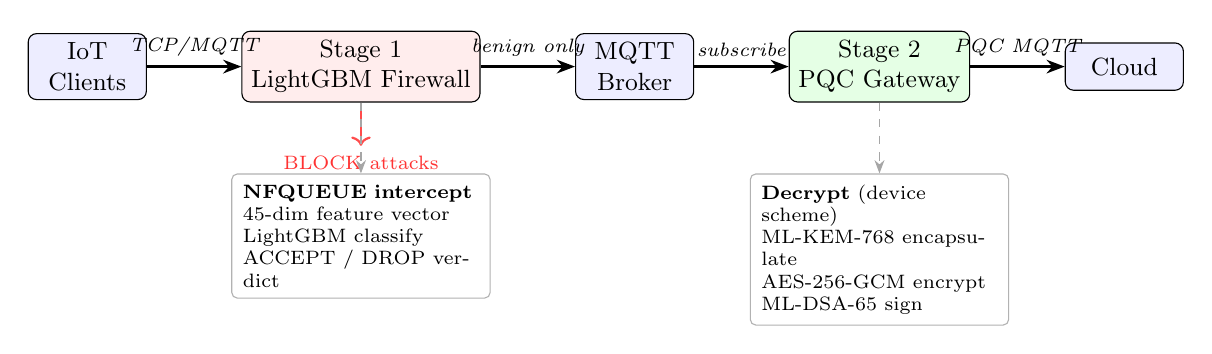
\begin{tikzpicture}[
    node distance=0.5cm and 0.4cm,
    box/.style={draw, rounded corners=3pt, fill=blue!7, minimum height=0.6cm,
                minimum width=1.5cm, font=\small, align=center},
    fwbox/.style={draw, rounded corners=3pt, fill=red!7, minimum height=0.6cm,
                  font=\small, align=center},
    gwbox/.style={draw, rounded corners=3pt, fill=green!10, minimum height=0.6cm,
                  font=\small, align=center},
    innerbox/.style={draw=gray!60, rounded corners=2pt, fill=white, font=\scriptsize,
                     align=left, text width=3.0cm, minimum height=1.4cm, inner sep=4pt},
    arr/.style={-Stealth, thick},
    darr/.style={-Stealth, dashed, gray!70},
    lbl/.style={font=\scriptsize\itshape, midway, above}
]

\node[box]   (iot)    {IoT\\Clients};
\node[fwbox, right=1.2cm of iot, minimum width=2.2cm] (fw) {Stage 1\\LightGBM Firewall};
\node[box, right=1.2cm of fw]  (broker) {MQTT\\Broker};
\node[gwbox, right=1.2cm of broker, minimum width=2.2cm] (gw) {Stage 2\\PQC Gateway};
\node[box,   right=1.2cm of gw]  (cloud)  {Cloud};

\draw[arr] (iot)    -- node[lbl]{TCP/MQTT} (fw);
\draw[arr] (fw)     -- node[lbl]{benign only} (broker);
\draw[arr] (broker) -- node[lbl]{subscribe} (gw);
\draw[arr] (gw)     -- node[lbl]{PQC MQTT} (cloud);
\draw[->, red!70, thick] (fw.south) -- ++(0,-0.55) node[below, font=\scriptsize, red!80]{BLOCK attacks};

\node[innerbox, below=0.9cm of fw] (fwdetail) {
    \textbf{NFQUEUE intercept}\\
    45-dim feature vector\\
    LightGBM classify\\
    ACCEPT / DROP verdict
};
\node[innerbox, below=0.9cm of gw] (gwdetail) {
    \textbf{Decrypt} (device scheme)\\
    ML-KEM-768 encapsulate\\
    AES-256-GCM encrypt\\
    ML-DSA-65 sign
};

\draw[darr] (fw.south) to[out=270,in=90] (fwdetail.north);
\draw[darr] (gw.south) -- (gwdetail.north);

\end{tikzpicture}
\caption{Two-stage IoT gateway security pipeline. Stage~1 blocks attack traffic at the network layer via LightGBM flow classification; Stage~2 upgrades surviving benign messages to NIST Level~3 PQC before cloud transit.}
\label{fig:arch}
\vspace{-4mm}
\end{figure*}

\subsection{Stage 1: LightGBM MQTT Firewall}

\textbf{Packet interception.} \texttt{iptables} rules redirect all TCP traffic on port~1883 into a Linux NetfilterQueue (NFQUEUE). The firewall process binds to this queue and processes each arriving packet via a \texttt{handle\_packet} callback that uses \texttt{dpkt} to decode IP and TCP headers. Critically, every packet is \textit{immediately accepted} back to the kernel before any classification runs, ensuring zero added latency to accepted MQTT sessions.

\textbf{Flow state and feature extraction.} The firewall maintains a bidirectional flow table keyed by the five-tuple \texttt{(src\_ip, dst\_ip, src\_port, dst\_port, protocol)}. Each entry accumulates per-direction packet counts, byte totals, packet-length lists, inter-arrival times, and cumulative TCP flag counts across the lifetime of the connection. Classification is triggered either by connection termination (FIN/RST with $\geq$3~packets) or periodically every 5~packets for long-lived connections such as publish floods. A background reaper thread classifies and removes flows idle for more than 10~seconds. Upon triggering, the flow record is converted into a 45-dimensional numerical feature vector covering: flow duration and packet rate; per-direction SYN/ACK/PSH/FIN/RST/ECE/CWR flag counts; protocol indicator bits; packet length statistics (total, min, max, mean, std); mean inter-arrival time; derived behavioral features (Magnitude, Radius, Covariance, Variance, Weight); and mean header length. The \textit{Weight} feature---the product of forward and backward packet counts---is particularly discriminative for flood attacks, where near-unidirectional traffic drives Weight toward zero.

\textbf{LightGBM classification.} The feature vector is normalized by a pre-fitted StandardScaler and submitted to a LightGBM gradient-boosted decision tree model~\cite{lightgbm2017} trained on the CIC IoMT~2024 dataset~\cite{ciciomt2024}, covering 21~traffic classes (benign plus 20~attack categories). A flow is labelled ATTACK if the predicted class is non-benign and benign-class probability falls below $1 - \tau$ (threshold $\tau = 0.5$). In IPS mode, confirmed attack source IPs are blocklisted for subsequent packets.

\subsection{Stage 2: PQC Gateway Re-Encryption}

The gateway subscribes to the MQTT broker and, for each received message, executes four steps: (S1)~decrypt the payload using the device's registered scheme (AES-256-GCM, Kyber-512+AES, etc.); (S2)~call \texttt{ML-KEM-768.encapsulate($pk_\text{cloud}$)} to obtain KEM ciphertext $c_\text{kem}$ and shared secret $ss$, then derive AES session key $k \leftarrow \text{HKDF-SHA256}(ss)$; (S3)~compute $c_\text{aes} \leftarrow \text{AES-256-GCM}_k(p, \eta)$ with a fresh 96-bit nonce; (S4)~compute $\sigma \leftarrow \text{ML-DSA-65.sign}(c_\text{kem} \| c_\text{aes} \| \eta,\; sk_\text{gw})$ and publish $\{c_\text{kem}, c_\text{aes}, \eta, \sigma\}$.

All keys are derived from a 256-bit master secret via HKDF-SHA256~\cite{rfc5869} scoped by algorithm and device ID---no key material is transmitted over MQTT. The scheme achieves IND-CCA2 confidentiality under ML-KEM-768 (NIST Level~3) and EUF-CMA integrity under ML-DSA-65 (NIST Level~3).

\textbf{Implementation.} Both stages run on a Raspberry Pi~4B (Broadcom BCM2711, 4~cores Cortex-A72 @ 1.8~GHz, 4~GB LPDDR4) under Python~3.11. The firewall uses \texttt{NetfilterQueue}, \texttt{dpkt}, and a pre-trained LightGBM model (\texttt{lightgbm\_model.txt}). The PQC gateway uses \texttt{liboqs-python}~0.10~\cite{oqs2023} for ML-KEM-768 and ML-DSA-65, the \texttt{cryptography} library for AES-256-GCM, and Paho-MQTT for broker communication. Timing is captured at nanosecond resolution via \texttt{time.perf\_counter\_ns()}, flushed asynchronously to avoid measurement perturbation.

\section{Experimental Evaluation}

\subsection{Setup}

\textbf{Stage~1 (IDS).} Synthetic attack traffic covering seven attack categories was injected in a controlled testbed. The firewall processed all traffic for approximately 75 seconds (02:02:18--02:03:33 UTC). Additionally, a dedicated 11-minute evaluation (10:42:43--10:53:29) injected 10~attack types to measure per-category timing.

\textbf{Stage~2 (PQC).} Three IoT client profiles---AES-256-GCM only, Kyber-512+AES, and ML-KEM-768+ML-DSA-65---ran concurrently, publishing at 2-second intervals. The gateway processed 144~benign MQTT messages over 20~minutes. All KEM and signature operations invoke real liboqs primitives; no simulation stubs are used.

\textbf{End-to-end.} A combined run spanning 20~minutes (09:37:26--09:57:23) exercised both stages simultaneously, injecting mixed attack and benign traffic.

\subsection{Stage 1: IDS Detection Performance}

Table~\ref{tab:ids} reports results from the primary IDS evaluation. Across 5,309~attack flows, the LightGBM model achieved \textbf{99.6\% attack detection} (5,309/5,329~flows) with a mean model confidence of \textbf{1.0000}; 100\% of detected attack flows exceeded the 0.90 confidence threshold. Zero attack flows reached the MQTT broker in IPS mode.

\begin{table}[!t]
\centering
\captionsetup{font=footnotesize, skip=2pt}
\caption{IDS Detection and Timing by Attack Category}
\label{tab:ids}
\footnotesize
\setlength{\tabcolsep}{3pt}
\begin{tabular}{lrrrr}
\toprule
\textbf{Attack Type} & \textbf{N} & \textbf{Conf.} & \textbf{Classify} & \textbf{Verdict} \\
                     &            & \textbf{Mean}  & \textbf{Mean (ms)}& \textbf{Mean (ms)} \\
\midrule
MQTT-DoS-Connect\_Flood  & 796 & 1.000 & 0.871 & 1.151 \\
MQTT-DDoS-Connect\_Flood & 16  & 1.000 & 1.958 & 2.521 \\
MQTT-DDoS-Publish\_Flood & 13  & 1.000 & 1.467 & 1.850 \\
MQTT-DoS-Publish\_Flood  & 8   & 1.000 & 1.189 & 1.379 \\
TCP\_IP-DDoS-SYN         & 13  & 1.000 & 1.491 & 1.713 \\
Recon-OS\_Scan           & 28  & 0.979 & 1.439 & 1.571 \\
TCP\_IP-DDoS-UDP         & 12  & 0.969 & 1.161 & 1.164 \\
ARP\_Spoofing / Other    & 7   & 0.978 & 1.875 & —      \\
\midrule
\textbf{Overall}         & 893 & 0.997 & \textbf{0.944} & \textbf{1.201} \\
\bottomrule
\end{tabular}
\vspace{-2mm}
\end{table}

\textit{Confidence} is the model's predicted attack-class probability. \textit{Classify} covers feature extraction + LightGBM inference + threshold decision. \textit{Verdict} is packet-arrival-to-verdict latency for connection-termination-triggered flows; reaper-triggered flows show no verdict latency (marked ---). The dominant category, MQTT-DoS-Connect\_Flood (89.1\% of flows), achieves the fastest classify time (0.871~ms) due to its simple, short-lived TCP patterns. Reconnaissance flows are slower (1.439~ms) because scan flows exhibit irregular IAT distributions that require more feature computation. The overall mean classify latency of 0.944~ms and verdict latency of 1.201~ms are well within MQTT session establishment windows ($\approx$50--200~ms), ensuring detection does not impede legitimate client reconnections.

\subsection{Stage 2: PQC Re-Encryption Latency}

Table~\ref{tab:pqc} reports gateway re-encryption latency across 144~messages.

\begin{table}[!t]
\centering
\captionsetup{font=footnotesize, skip=2pt}
\caption{Gateway PQC Re-Encryption Latency (Real liboqs, $N=144$)}
\label{tab:pqc}
\footnotesize
\setlength{\tabcolsep}{3.5pt}
\begin{tabular}{lrrrr}
\toprule
\textbf{Stage} & \textbf{Mean} & \textbf{Std} & \textbf{P95} & \textbf{Max} \\
\midrule
ML-KEM-768 encapsulate & 0.047 ms & 0.019 ms & 0.065 ms & 0.215 ms \\
AES-256-GCM encrypt    & 0.030 ms & 0.143 ms & 0.024 ms & 1.609 ms \\
ML-DSA-65 sign         & 0.113 ms & 0.052 ms & 0.221 ms & 0.286 ms \\
\midrule
\textbf{Total re-encrypt}   & \textbf{0.189 ms} & 0.176 ms & 0.297 ms & 1.979 ms \\
On-device handler           & 0.488 ms & 0.981 ms & 0.613 ms & 11.5 ms \\
\bottomrule
\end{tabular}
\vspace{-2mm}
\end{table}

ML-KEM-768 encapsulation averages 47~$\mu$s (std~19~$\mu$s), reflecting the efficiency of lattice-based KEMs on ARM Cortex-A72. ML-DSA-65 signing at 113~$\mu$s is the dominant crypto cost, expected given the 2.4~KB signing key~\cite{nist_fips204}. AES-256-GCM exhibits mean~$>$~P95 (30~$\mu$s vs.\ 24~$\mu$s), a heavy-tailed distribution caused by rare OS-scheduling preemptions; the typical path (P95) is consistently under 24~$\mu$s. Total re-encrypt P95 of 0.297~ms is negligible relative to a 2-second publish interval. The on-device handler mean of 0.488~ms includes MQTT callback dispatch, JSON parsing, and HKDF key setup; its high standard deviation (0.981~ms) reflects OS jitter, not cryptographic variability.

\subsection{End-to-End Pipeline}

In the combined run, 5,481~packets generated 37~flow verdicts, of which 36~were attacks (97.3\% detection rate). The single benign flow's 144~messages were successfully re-encrypted. No attack traffic reached the gateway (0~firewall misses). The mean LightGBM inference latency in this run was 0.906~ms, and the mean full gateway handler time was 0.488~ms---confirming that both stages operate within the same latency budget and do not compound each other's jitter when pipelined.

Table~\ref{tab:e2e} summarizes the end-to-end pipeline characteristics.

\begin{table}[!t]
\centering
\captionsetup{font=footnotesize, skip=2pt}
\caption{End-to-End Pipeline Summary}
\label{tab:e2e}
\footnotesize
\setlength{\tabcolsep}{4pt}
\begin{tabular}{lrr}
\toprule
\textbf{Metric} & \textbf{Stage 1 (IDS)} & \textbf{Stage 2 (PQC GW)} \\
\midrule
Flows / Messages processed    & 37 flows       & 144 messages \\
Attack detection rate         & 97.3\%          & — \\
Firewall misses (attacks)     & 0              & — \\
Mean inference / re-encrypt   & 0.906 ms       & 0.189 ms \\
Mean full handler latency     & —              & 0.488 ms \\
PQC algorithm                 & —              & ML-KEM-768 + ML-DSA-65 \\
Security level                & —              & NIST Level 3 \\
Hardware                      & \multicolumn{2}{c}{Raspberry Pi 4B (real liboqs)} \\
\bottomrule
\end{tabular}
\vspace{-4mm}
\end{table}

\section{Discussion}

\subsection{Why the Two Stages Compose}

The two stages address different failure modes and therefore compose naturally at the gateway. Stage~1 acts before broker admission, where volumetric MQTT floods, scan traffic, and spoofed connection attempts can still be dropped cheaply using flow-level statistics. Stage~2 acts only after broker delivery, where the message has already passed the network-policy boundary and can be upgraded cryptographically for cloud transit. This separation avoids applying expensive PQC operations to traffic that the IDS has already identified as malicious, while also avoiding dependence on the IDS for long-term confidentiality.

The measured latencies support this design. Stage~1 inference remains near 1~ms per classified flow, which is small relative to TCP connection setup and MQTT session establishment. Stage~2 adds 0.189~ms of mean cryptographic overhead per accepted message, which is three orders of magnitude smaller than the 2-second publish interval used in the testbed. Even when both stages execute in the same 20-minute run, their timing paths remain independent: the firewall verdict loop handles packets and flows, while the PQC gateway handles broker-delivered application messages.

\subsection{Deployment Implications}

For operators, the main benefit is incremental deployability. Existing sensors can continue using their current device-side credentials and MQTT client libraries, while the gateway enforces two upgrades at the network boundary: attack filtering before broker admission and NIST Level~3 protection before cloud forwarding. This is particularly useful for brownfield deployments where endpoint firmware updates are slow, risky, or impossible. It also localizes policy changes to the gateway, allowing the IDS model, blocklist threshold, PQC parameter set, or cloud topic structure to be changed without touching every device.

The primary operational trade-off is bandwidth rather than latency. The fixed 4,425-byte PQC expansion is acceptable for gateway-to-cloud Ethernet, Wi-Fi, or 5G uplinks, but would be inappropriate on low-power device links. The proposed placement intentionally keeps that cost off constrained networks: devices send the original MQTT payload to the local broker, and only the upgraded cloud-bound message carries the ML-KEM ciphertext and ML-DSA signature. In deployments with smaller payloads or expensive backhaul, batching, compression before encryption, or policy-based selective upgrading may further reduce uplink cost.

\section{Conclusion}

We presented a two-stage IoT security pipeline combining a LightGBM MQTT intrusion detection system with a post-quantum gateway re-encryption stage, both implemented and measured on real Raspberry Pi~4B hardware. Stage~1 detected 99.6\% of attack flows (5,309 out of 5,329) with mean confidence~1.0000 and a mean classify latency of 0.944~ms. Stage~2 re-encrypted 144~benign MQTT messages with a mean total crypto overhead of 0.189~ms using NIST Level~3 ML-KEM-768 and ML-DSA-65 via genuine liboqs primitives. In the end-to-end evaluation, zero attack messages reached the PQC gateway, confirming that the two stages compose cleanly without introducing additional latency coupling.

\textbf{Limitations.} The IDS model was trained on the CIC IoMT~2024 dataset and may require retraining for deployment environments with different traffic distributions. WAN transit time between the gateway and cloud was not measured; clock skew between nodes warrants calibration in multi-Pi deployments. The Python runtime introduces per-call overhead (JSON parsing, Paho-MQTT dispatch) that is absent in a C/C++ production implementation.

\textbf{Future Work.} We plan to extend the evaluation to a distributed four-node Raspberry Pi network with heterogeneous payload sizes (5~KB--100~KB), integrate TLS-over-MQTT on the cloud-facing segment, and explore hardware acceleration of ML-KEM-768 on the Raspberry Pi~4B's Cortex-A72 NEON SIMD units. Adversarial robustness of the LightGBM model against evasion attacks will also be investigated.

\section*{Acknowledgment}
This work was partly supported by IITP grants funded by the Korea government (MSIT): the Innovative Human Resource Development for Local Intellectualization Program (IITP-2026-RS-2020-II201612, 34\%) and the ITRC Program (IITP-2026-RS-2024-00438430, 33\%); and by the Basic Science Research Program through NRF, funded by the Ministry of Education (2018R1A6A1A03024003, 33\%).

\balance
\bibliographystyle{IEEEtran}
\bibliography{references_4page}

\end{document}
